\documentclass{article}
\usepackage[utf8]{inputenc}
\usepackage{CJKutf8}

\title{CS224N-PA1}
\author{Name: Jiawei Yao \quad SUNetID: jwyao \\ Name: Wei Wei \quad SUNetID: wwei2}
\date{\today}

\usepackage{graphicx}
\usepackage{caption}
\usepackage{subcaption}
\usepackage{geometry}
 \geometry{
 a4paper,
 total={210mm,297mm},
 left=20mm,
 right=20mm,
 top=20mm,
 bottom=20mm,
 }
\usepackage{parskip}

\begin{document}

\maketitle

\section{Word Alignment}

\subsection{Evaluation}

We use 10k sentences as the training and produced evaluation results as follows. As is shown in Table~\ref{tab:dev} and Table~\ref{tab:test}, we can see that Model 2 has a lot better performance than model 1 and PMI when it comes to French-English translation and Chinses-English translation. As for Hindi-English, model 1 is slightly better than model 2 and far more better than PMI model.

\begin{table}[!htb]
\centering
\begin{tabular}{cccc}
 \hline
 & French-English & Hindi-English & Chinese-English \\
 \hline
 PMI & 0.7127 & 0.8594 & 0.8258 \\
 Model 1 & 0.3544 & 0.5823 & 0.5869 \\
 Model 2 & 0.3129 & 0.6048 & 0.5770 \\
 \hline
\end{tabular}
\caption{AER for dev}
\label{tab:dev}
\end{table}

\begin{table}[!htb]
\centering
\begin{tabular}{cccc}
 \hline
 & French-English & Hindi-English & Chinese-English \\
 \hline
 PMI & 0.6917 & 0.8213 & 0.8090 \\
 Model 1 & 0.3494 & 0.5802 & 0.5862 \\
 Model 2 & 0.3013 & 0.5990 & 0.5648 \\
 \hline
\end{tabular}
\caption{AER for test}
\label{tab:test}
\end{table}

\subsection{Development Issues}

\paragraph{Interesting details}
\begin{enumerate}
\item In Collin's notes, the M-step in Model 1 parameter estimation also updates $q(j|i,l,m)$, which is unnecessary and caused some confusion.
\item It took us some time to figure out the notation of aligning target to source, which is slightly different from the lecture slides and Collin's notes. After figuring out the right formula, coding is easy.
\item \texttt{CounterMap} and \texttt{Counters.conditionalNormalize()} are helpful.
\item It's difficult for our models to converge. With 10K training data, we tried a maximum iterations of 100 for Model 1 and 75 for Model 2. Neither converged.
\item However, increasing number of iterations doesn't help reduce AER. On the contrary, we found early stopping helpful by setting iterations to 20.
\item There might be an issue with unknown word, which would lead to division by zero error. However, during our tests, this problem never happened.
\end{enumerate}

\paragraph{Convergence criterion} Let $t_{k}(e_i, f_j)$ and $q_{k}(a_i|i, n, m)$ denote $t(e_i, f_j)$ and $q(a_i|i, n, m)$ in $k$th iteration. When $|t_{k - 5}(e, f) - t_{k}(e, f)| <= 10^{-4}$ and $q_{k -5}(a_i|i, n, m) - q_{k}(a_i|i, n, m) <= 10^{-4}$, we decide it is converged. As an optimization, we check convergence every five iterations to avoid excessive computation as each check is expensive.
\paragraph{Number of iterations} We run 20 iterations for Model 1 and 20 iterations for Model 2 training. We discovered that running more iterations can help performance but don't help much and it takes more time.

\subsection{Error Analysis}

Let's evaluate our alignment model by looking at a specific example. It's the 22nd sentence pair of Chinese and English corpus since we are native Chinese speakers. The alignment result is visualized using Picaro (the red cells indicate wrong alignments) in Figure~\ref{fig:alignment}.

\begin{figure}[!htb]
\centering
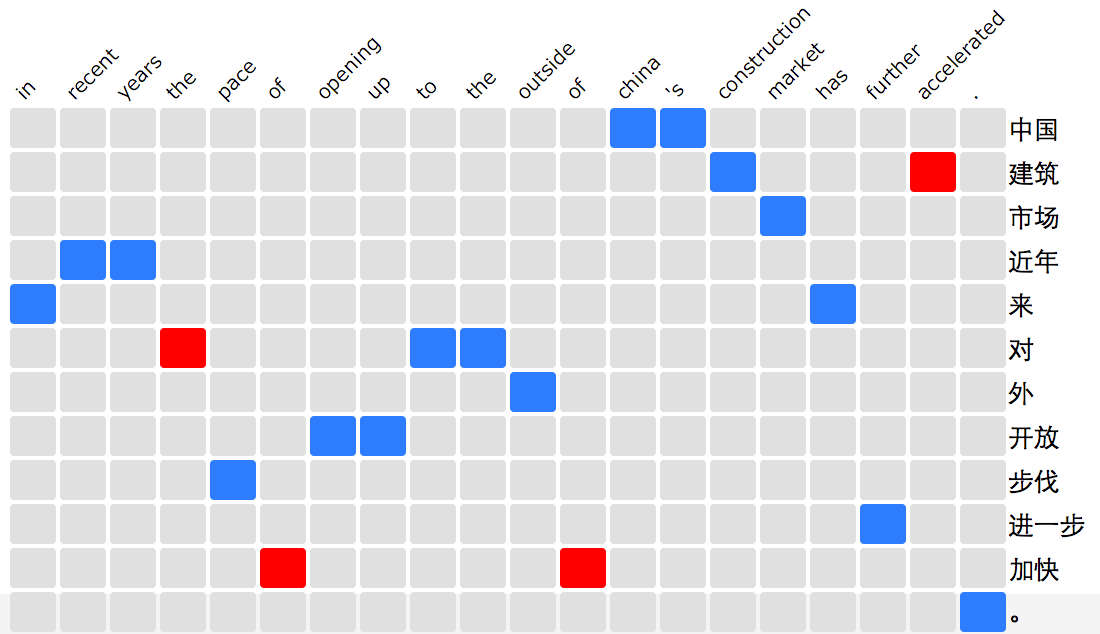
\includegraphics[width=.9\textwidth]{alignment}
\caption{Example Alignment}
\label{fig:alignment}
\end{figure}

Let's discuss the alignment in different aspects:

\begin{CJK*}{UTF8}{gbsn}

\begin{itemize}
\item \textbf{Word Order} For this sentence pair, the alignment is totally out of order, with only a few alignments in the main diagonal. However, in general our alignment model had no problem handle word order differences.
\item \textbf{Function Words} There are a few English function words in the English sentence (in, of, to) and a few Chinese function words (来, 对). Our model has mixed quality when aligning function words. For example, since 来 in Chinese means ``after (some time)", aligning it to ``has", which means a perfect tense, is plausible. But the ``of" in ``the pace of" is mis-aligned to 加快, which is a verb in Chinese. Actually, ``the pace of" should be aligned to 步伐. This shows the why phrase translation is superior to word-based translation.
\item \textbf{Mistakes} There are four mistakes in this alignment: two for function words and two for aligning ``accelerated" to ``加快". And three of them is related to ``加快". We guess maybe ``加快" doesn't appear frequently in this corpus (there are alternate translations for accelerate, e.g. 加速) so the conditional probability is very low.
\end{itemize}

\paragraph{Common Mistakes} Beyond this particular example, the most common mistakes we observe in the alignments generated by our model (IBM Model 2) include mis-aligning of function words, mis-aligning from missing corresponding part, aligning multiple English words to a single Chinese word, mis-aligning from abbreviations, mis-alinging from uncommon target words, different representations of numbers and dates, misaligning from break of phrases by inaccurate segmentation, etc.

\clearpage\end{CJK*}

\section{Machine Translation}

\subsection{BLEU Scores}

\begin{table}[!htb]
\centering
\begin{tabular}{c|c|c|c}
\hline
 Feature & Average BLEU & Best BLEU & Lowest BLEU\\
\hline
 cs224n-staff & 15.000 & - & -\\
 baseline & 15.210 & 15.464 & 15.140\\
 number & 15.446 & 15.644 & 15.270 \\
 of & 15.348 & 15.671 & 15.042 \\
\hline
\end{tabular}
\caption{BLEU Score for MT}
\label{tab:bleu}
\end{table}

\paragraph{Note} BLEU scores for each feature set are based on 5 runs.

\subsection{New Feature 1: Numbers}

\paragraph{Motivation} Our key motivation for this feature is that after we run the baseline system, we discovered a lot of differences associated with numbers between baseline and reference system. Differences are shown in Table~\ref{tab:baselinevsreference}. We wouldn't say these baseline translations are bad but we believe they hurt BLEU score. 12,000 is essentially the same as 12 thousand but there is no thousand in baseline translation its performance will be affected. Given the discovery we make, we are motivated to improve the BLEU score by incorporating this number feature into the system.

\begin{table}[!htb]
\centering
\begin{tabular}{c|c}
\hline
 Baseline & Reference \\
\hline
 individual countries released their \textbf{3q gdp} data  & each state has published the information to \textbf{gdp 3 a} \\
 the yield on \textbf{ten-year} bonds on is by 28.45 \% & the earnings on its \textbf{10-year} bonds are 28.45 \% \\
 it is more than \textbf{12,000} students & joined by over \textbf{12 thousand} school children \\
\hline
\end{tabular}
\caption{Translation Differences between Baseline and Reference}
\label{tab:baselinevsreference}
\end{table}

\paragraph{Implementation} We create an indicator feature that considers the \textit{difference} between the number of numbers appeared in source phrase and target phrase. If source phrase contains a ``10'' but target phrase contains ``ten'', we will add a feature \textsc{NUMBER:1} with value 1.0 to this phrase pair. If source phrase doesn't contain numbers but target phrase contains a ``10'', then we fire a feature \textsc{NUMBER:-1} with value 1.0. If there are same number of numbers appeared in target phrase and source phrase, we fire a feature \textsc{NUMBER:0} with value 1.

\paragraph{Results} By implementing this new feature, we are happy to observe that there are several sentences that this feature helps a lot. The comparison is shown at Table~\ref{tab:baselinevsnumber}.

\begin{table}[!htb]
\centering
\begin{tabular}{c|c}
\hline
 Baseline & Number \\
\hline
 individual countries released their \textbf{3q gdp} data  & each state has published the information to \textbf{gdp 3 a} \\
 the yield on \textbf{ten-year} bonds on is by 28.45 \% & the return on the obligations on \textbf{10 years} is by 28.45 \% \\
\hline
\end{tabular}
\caption{Translation Differences between Baseline and Number}
\label{tab:baselinevsnumber}
\end{table}

\subsection{New Feature 2: OF}

\paragraph{Motivation} The motivation for this feature is that after comparing the baseline translations with the reference translations, we found that the baseline translations tend to favor phrases with ``of". See the example below for reference. An excessive using of ``of" is wordy and reduces sentence fluency. As a result, we decide that an appearance of ``of" in the target phrase might be a good indicator.

[\textbf{Reference}] within \textbf{the code of} criminal procedure amendment , the motion to revoke an article based on which the opposition leader , yulia tymoshenko , was sentenced

[\textbf{Baseline}] \textbf{in the context of} an amendment to the criminal law , \textbf{the project of} \textbf{the cancellation of} the paragraph establishing \textbf{the charges of} julia tymosenko , \textbf{the head of} the opposition

\paragraph{Implementation} We create an indicator feature that considers the \textit{number} of ``of"'s appearing in the target phrase. For example, if the target phrase contains two ``of"'s , we will add a feature \textsc{NUMOF:1} with value 1.0 to this phrase pair.

\paragraph{Results} After implementing ``of'' feature, we discovered that the number of ``of'' decreased and our system tends to use words that are more meaningful than ``of'' so that we can achieve higher BLEU score. For example, our system outputted ``the germany 's gdp growth expected 0.5 \% , that of france by 0.4 \%'' while baseline system translated as ``the germany 's gdp growth expected 0.5 \% , that of france of 0.4 \% .''. Instead of ``of'', our system uses ``by'' and it is exactly the same as the reference text.

\subsection{Other Features}

The following features might be useful but we didn't take time to try them:

\begin{enumerate}
\item \textbf{Part of Speech} If we can mark the POS of both the source and target word, we can guide the searching to glue words of the same POS together. However, determining the POS tags of a word is not trivial. This task is even harder considering phrases.
\item \textbf{Tense} When comparing the baseline and reference translations, we found that the baseline translations have a non-trivial possibility of wrong tense. If we can add an indicator of tense given some indicative pattern (e.g. ``has [verb-ed]", ``[be] [verb-ing]"), we might have better translations.
\item \textbf{Sentence Length Difference} We assume that for similar languages, e.g. French and English, the original and target translation should have a similar sentence length. Therefore we can add an indicator feature of the absolute value of sentence difference. However, this feature might not generalize to other languages, such as Chinese-to-English and Japanese-to-English.
\end{enumerate}

\section{Extra Credit}

\subsection{Scalability}

We used our original code and tested it against larger corpus and had fairly good performance. the training time is proportional to the size of the training corpus so we can safely make the conclusion that our code scales well. We ran 5 iterations of Model 1 and 1 iteration of Model 2 and the result is shown in Figure~\ref{fig:scale} and Figure~\ref{fig:aer}. AER significantly drops as we increase the size of the training corpus and it can reach its lowest 0.2534 using 100k iterations.

\begin{figure}[!htb]
\centering
\begin{subfigure}[b]{0.45\textwidth}
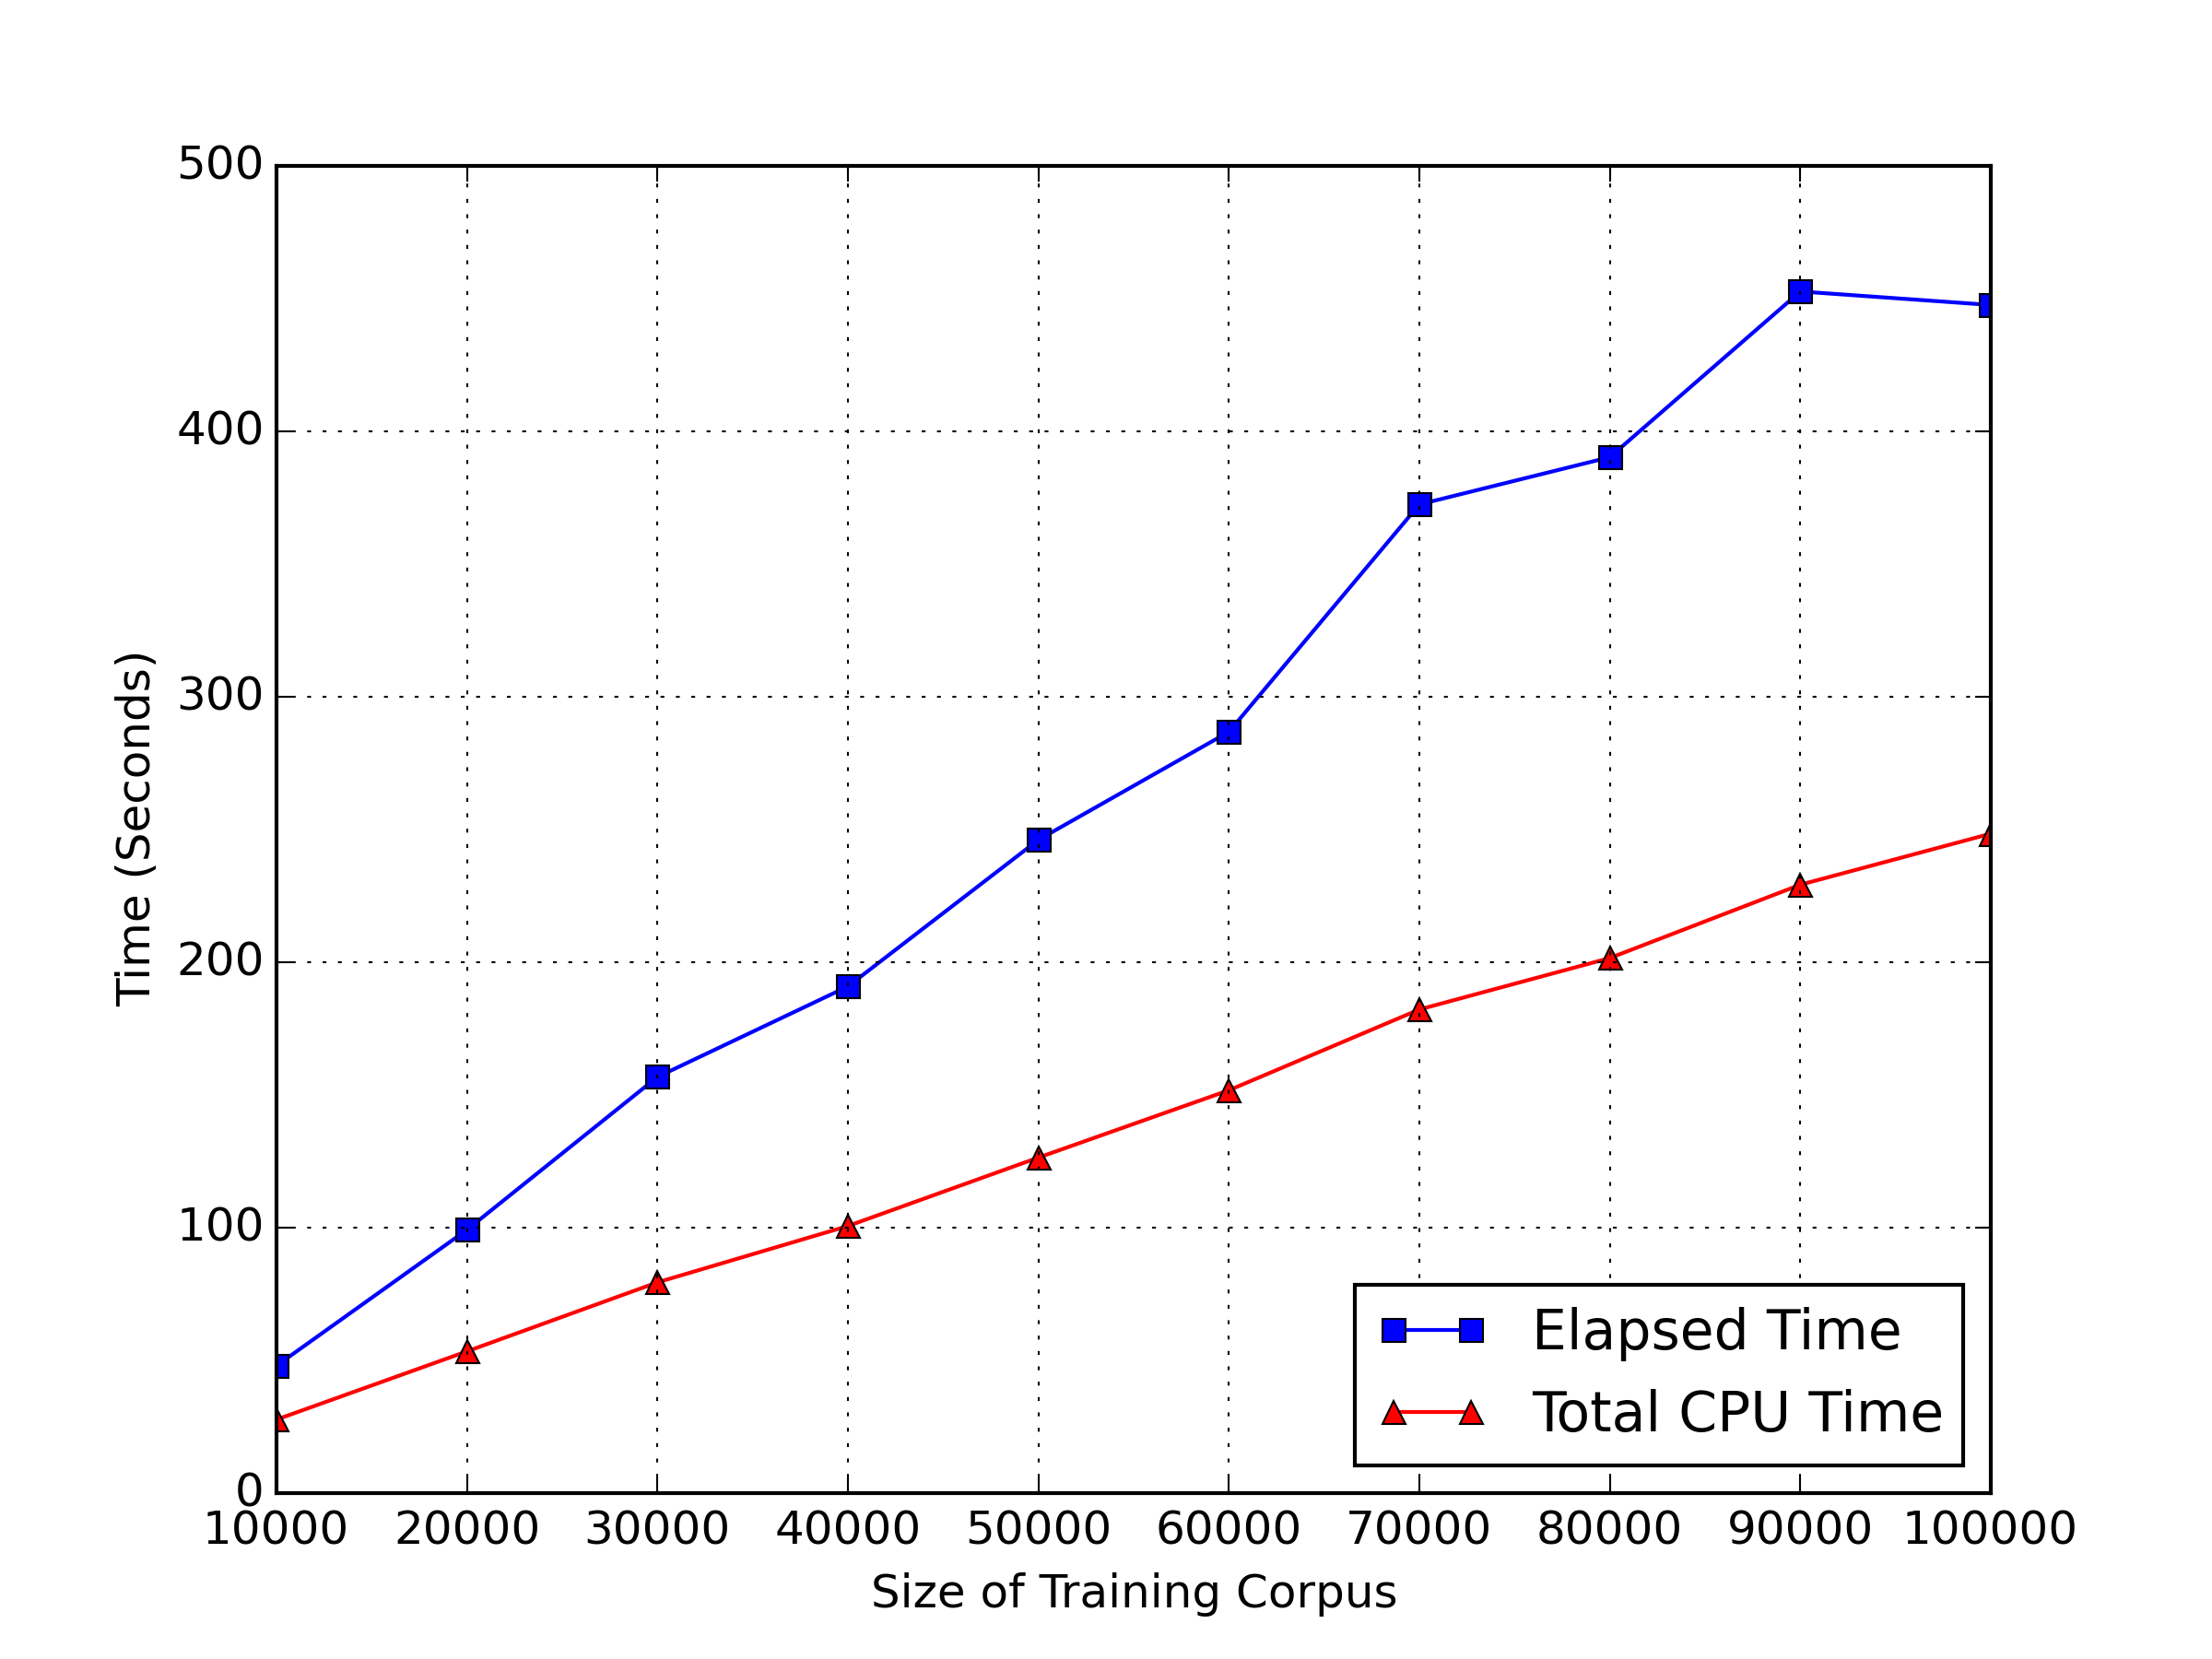
\includegraphics[width=\textwidth]{time}
\caption{Scalability}
\label{fig:scale}
\end{subfigure}%
~ %add desired spacing between images, e. g. ~, \quad, \qquad, \hfill etc.
%(or a blank line to force the subfigure onto a new line)
\begin{subfigure}[b]{0.45\textwidth}
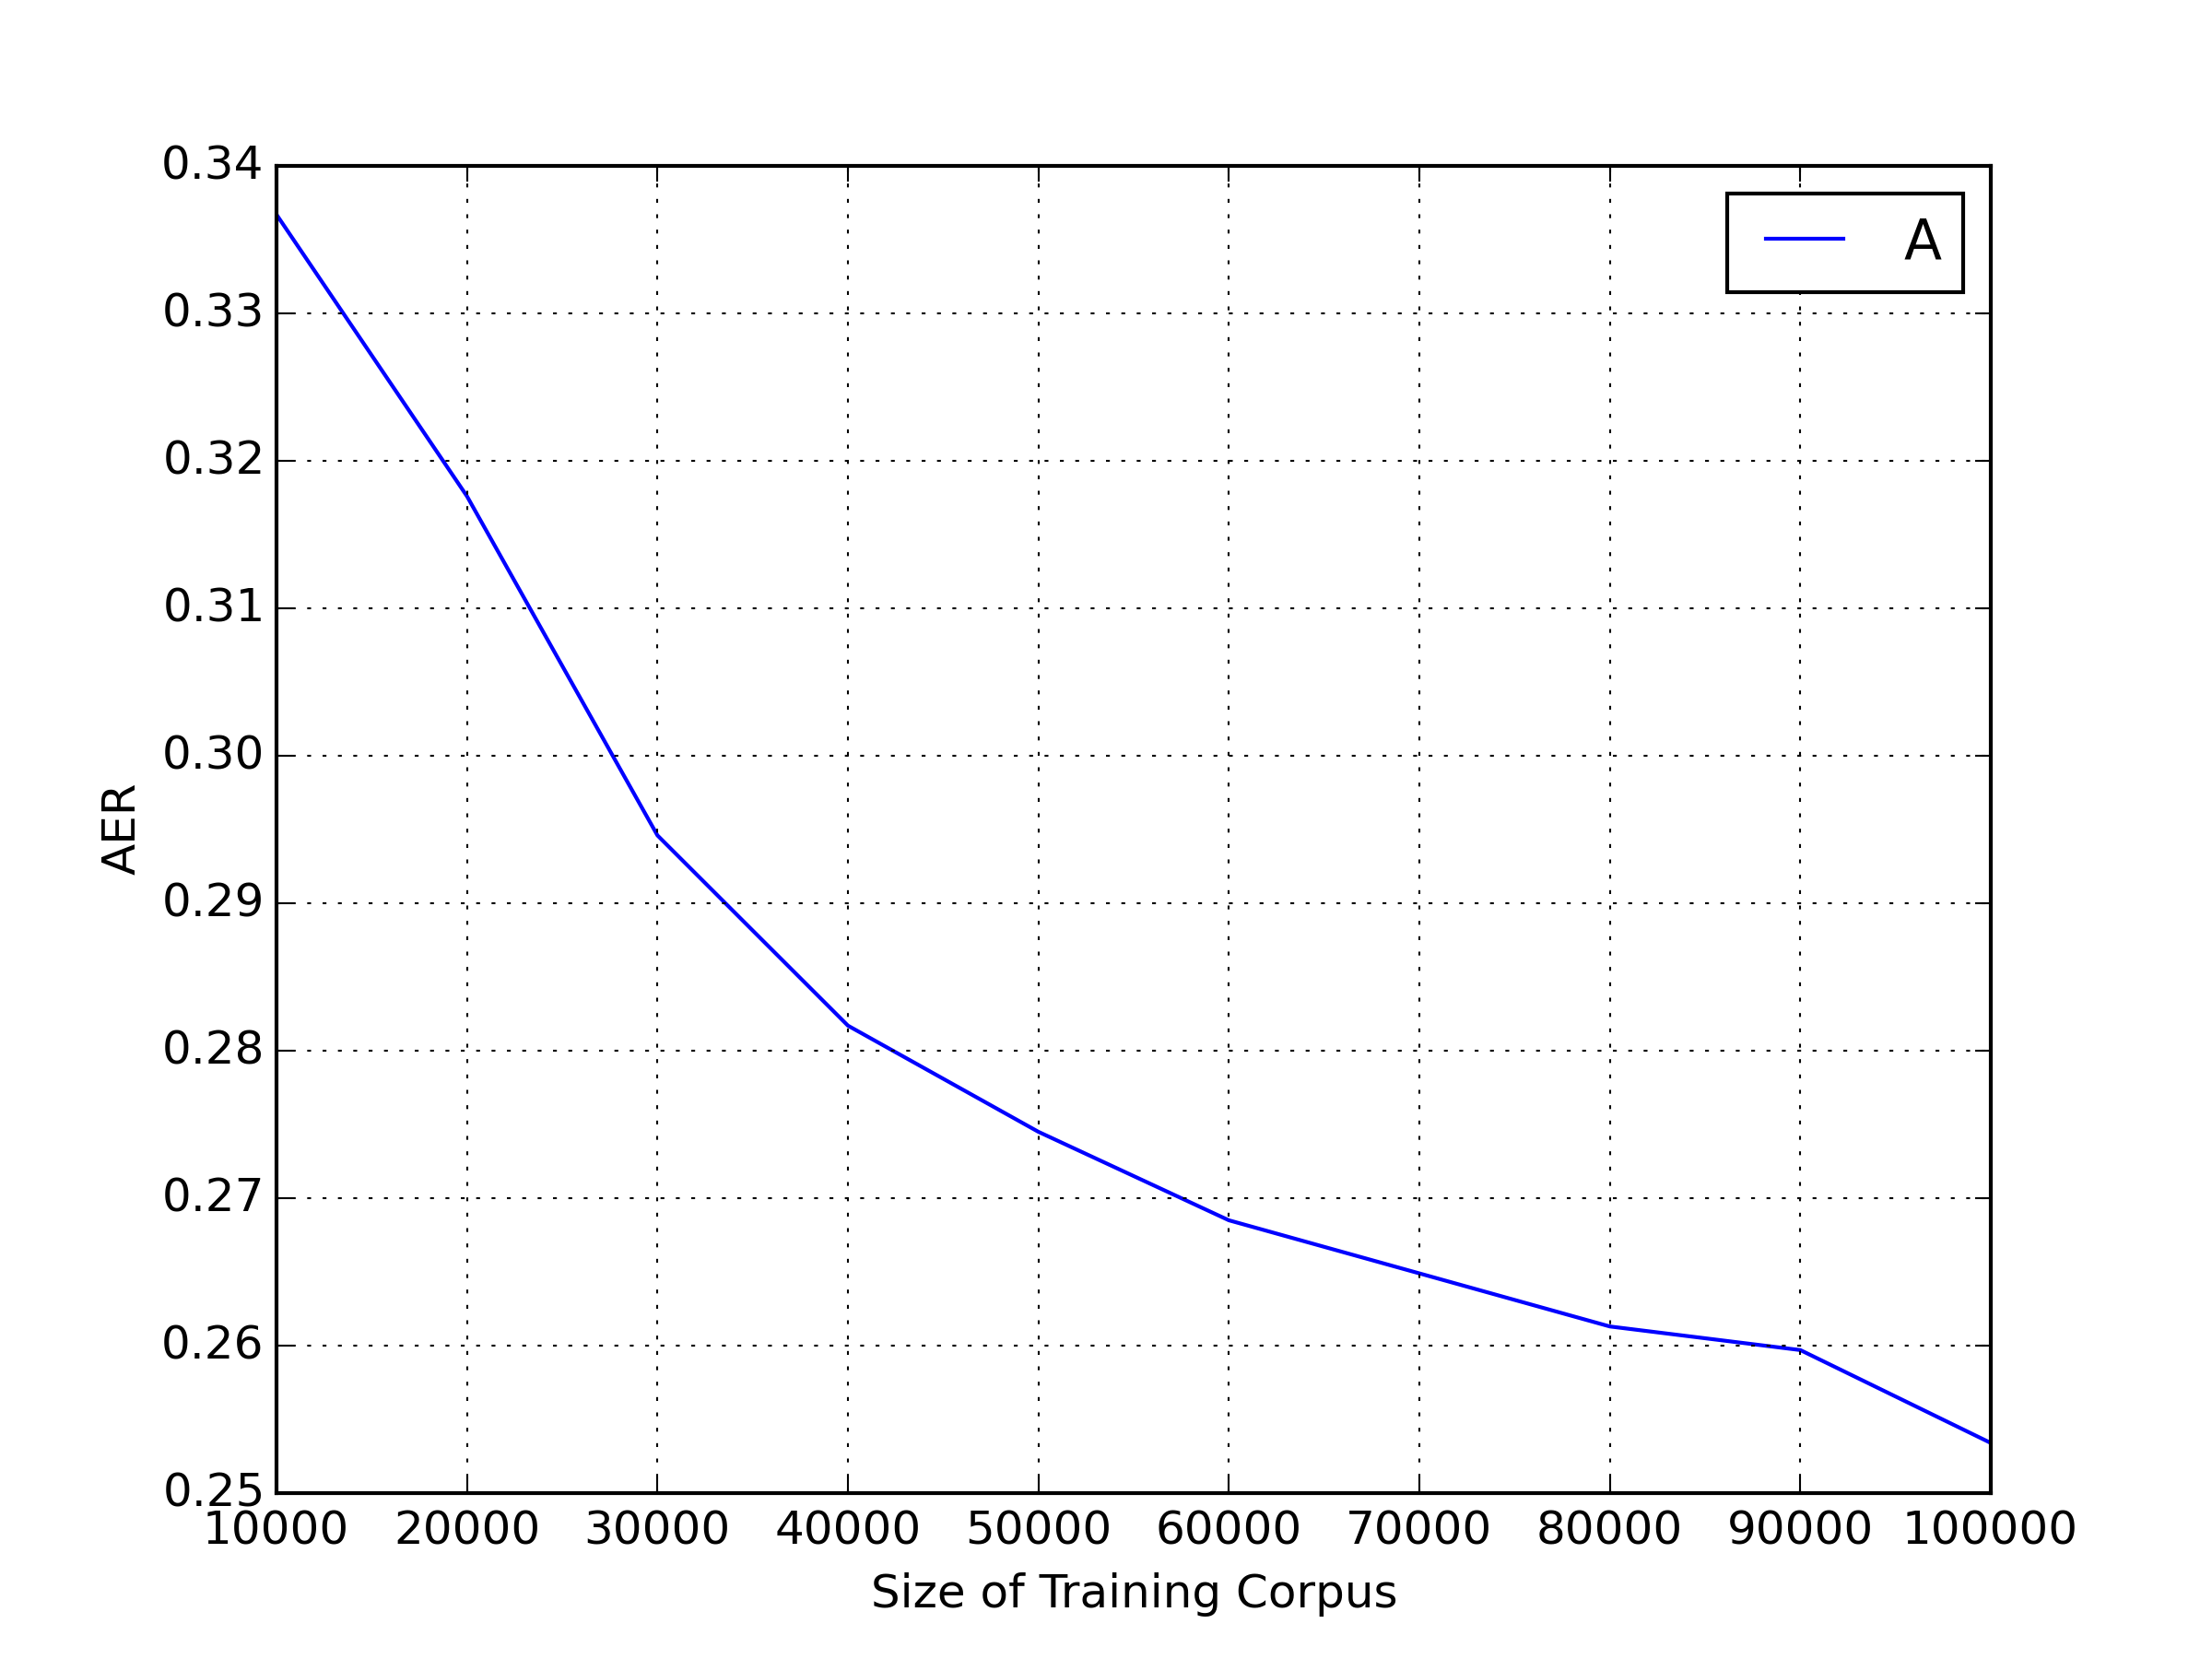
\includegraphics[width=\textwidth]{aer}
\caption{AER}
\label{fig:aer}
\end{subfigure}
\end{figure}

\subsection{Comparison between Phrasal and Google Translate}

We selected about 30 sentences from our translations and compared it with Google's translation. For most of the time, Google's translation is better and you can have a look at it at \textit{extra.txt}. Errors are categorized as follows.

\subsubsection{Error Categories}

\paragraph{wrong singular, plural form}
\begin{description}
\item[Google:] among their favorite dishes there are a lot of cakes, meats and sweets.
\item[Phrasal:] among their favourite meals there \textit{is} a lot of cakes , meat and sweets .
\end{description}

\paragraph{missing verbs; bad fluency}
\begin{description}
\item[Google:] the designer must know how optically ammenuiser wide arm, \textit{extend} the neck or add curves required.
\item[Phrasal:] the designer must know how optically arm wide , a neck or add curves necessary .
\end{description}

\paragraph{wrong collocation, consecutive nouns}
\begin{description}
\item[Google:] this time we have with the director alenka (over there no boys) treated the way to dress the woman who has no standard measurements.
\item[Phrasal:] this time we have with the director alenka ( \textit{in there} is no boy ) treaty of how to dress the woman who has no \textit{measurements standards} .
\end{description}

\paragraph{bad grammatical structure}
\begin{description}
\item[Google:] or simply holding sleeves or neck and immediately have a new look.
\item[Phrasal:] or enough to walk up the collar , \textit{sleeves or immediately and} have a new look .
\end{description}

\paragraph{wrong subject}
\begin{description}
\item[Google:] for example in the desert you find yourself in a sand storm that reduces your visibility significantly.
\item[Phrasal:] for example in the desert you find yourself in a sandstorm \textit{you} declines significantly the visibility .
\end{description}

\paragraph{missing critical subject}
\begin{description}
\item[Google:] mario made me happy when \textit{he} congratulated me on my creation.
\item[Phrasal:] mario i was glad when congratulated me for my creation .
\end{description}

\paragraph{better brevity}
\begin{description}
\item[Google:] originally a trouble-free race turns because of a series of stupid mistakes of people who don 't have anything to do routine work morning shift.
\item[Phrasal:] originally a race without problem due to a set of stupid mistakes with people who \textit{have nothing to do} in a routine early to work .
\end{description}

\paragraph{wrong translation}
although prêts by itself means ``be ready to", in this context it should be translated to ``be willing to".
\begin{description}
\item[Source:] l' enquête a montré également que les enfants sont prêts à changer leurs habitudes à partir du moment où ils reçoivent les informations ad hoc .
\item[Google:] the survey also found that children are willing to change their habits from the time they receive adequate information.
\item[Phrasal:] the survey showed that children are \textit{ready to} change their habits if they receive information \textit{ad hoc} .
\end{description}

\end{document}
